\documentclass[12 pt,a4paper]{report}
\usepackage{graphicx}
\usepackage{fancyhdr}
\pagestyle{fancy}
\usepackage{ragged2e}
\usepackage{comment} 
\usepackage{listings}
\usepackage{amsmath}
\usepackage[export]{adjustbox}
\usepackage[usenames,dvipsnames]{color}
\usepackage[utf8]{inputenc}
%\usepackage{blindtext}
\pagenumbering{roman}
\begin{document}
\begin{titlepage}
\begin{center}
\hspace{1 cm} A PROJECT REPORT ON 
\vspace{1 cm}
\\
\textbf{“A Feedback Management System”} 
\vspace{1 cm}
\\
Submitted in partial fulfillment of the requirements 
\vspace{0.5 cm}
\\
of the degree of
\vspace{1 cm}
\\
\textbf{B.TECH IN COMPUTER ENGINEERING}
\vspace{0.5 cm}
\\
BY
\vspace{0.5 cm}
\\
\textbf{Mr. Shivsamb Chonde}\\
\textbf{Mr. Sagar Mayekar}\\
\textbf{Mr. Ajaykumar Chavan}
\vspace{0.5 cm}
\\
Under the guidance
\vspace{0.6 cm}
\\
of 
\vspace{0.6 cm}
\\
\textbf{Prof. Hansraj Wankhede}
\\  
\textbf{Ms. Pranita Jadhav}  
\\

\begin{center}

\includegraphics[scale=.7]{logo.png}
\vspace{1 cm}
\\
\textbf{DEPARTMENT OF COMPUTER ENGINEERING}
\vspace{0.5 cm}
\\
Dr.Babasaheb Ambedkar Technological University,
\\
LONERE,Dist. Raigad Pin-402103(MS)
\\
\textbf{Academic Year 2016-2017}
\end{center}
\end{center}
\end{titlepage}
\newpage
\rhead{Feedback management System}
\lfoot{Dr.Babasaheb Ambedkar Technological University, Lonere }
\lhead{ }
\cfoot{ }
\rfoot{Page \thepage}
\hspace{0.2 cm}
\center\textbf{Academic Year 2016-2017}
\vspace{0.5 cm}
\\
\flushleft 
{\large \textcolor{Red}{Dr.Babasaheb Ambedkar Technological University,}}
 \\
{\large \textcolor{Red}{LONERE,Dist. Raigad Pin-402103(MS)}}
 \\
{\large \textcolor{Red}{Department of Computer Engineering}}  
 \\
 \begin{center}
 \flushright
 \vspace{-3 cm}

\includegraphics[scale=.7]{logo.png}
\end{center}

\begin{center}
\vspace{1.0 cm}
\rule{\textwidth}{2 pt}
\flushleft
\flushleft Date:\hspace{6 pt} / \hspace{5 pt} /
\\
\center\textbf{CERTIFICATE}
\\
\vspace{1 cm}
\justify
This is to certify that \textbf{Shivsamb Chonde}, \textbf{Sagar Mayekar},\textbf{Ajaykumar Chavan} has successfully submitted his project report on “Feedback Management System ” at in the partial fulfillment of the Graduate Degree course in\textbf{ B.Tech In Computer Engineering} at the Department of Computer Engineering, in the academic Year 2016-2017 (Semester-VI) as prescribed by the DBATU.\\

{\vspace{1in}}
    \vfill
    \begin{tabular}{ccc}
      \rule{5cm}{1sp} & \rule{12mm}{0pt} & \rule{5cm}{1sp} \\
{Ms. Pranita Jadhav} &&{Prof. Dr. Arvind Kiwelekar} \\
      {\textbf{Guide}} && {\textbf{HOD}}\\ 
      {(Computer Engineering)}&& {( Computer Engineering)}\\  
{\vspace{1in}}        
\rule{5cm}{0sp} & \rule{12mm}{0pt} & \rule{5cm}{0sp} \\          
\rule{5cm}{1sp} & \rule{12mm}{0pt} & \rule{0cm}{1sp} \\
{Prof Hansraj Wankhede} \\
      {\textbf{Subject Teacher}} \\ 
      {(Computer Engineering)}  
 
    
      \end{tabular} 
\end{center}


\newpage
\begin{center}
\textbf{Acknowledgement}
\justify
Apart from the efforts of us, the success of any project depends largely on the encouragement and guidelines of many others. We take this opportunity to express our gratitude to the people who have been instrumental in the successful completion of this project.\par
\justify
It is my immense pleasure to express my gratitude to Ms. Pranita Jadhav as guide who provided me constructive and positive feedback during the preparation of this seminar. I express my sincere thanks to the head of department Dr. A W KIWELEKAR (Computer Engineering) and all other staff members of Computer Department for their kind co-operation.\par 
\justify
The guidance and support received from all the members who contributed
and who are contributing to this project, was vital for the success of the project. 
We are grateful for their constant support and help.
\flushright \textbf{Shivsamb Chonde  (20150677)}
\flushright\textbf{Sagar Mayekar (20150684)}\flushright\textbf{Ajaykumar Chavan (20150676)}

\end{center}
\newpage
\begin{center}
\textbf{Abstract}
\justify
We developed software called feedback management system for computer engineering department. Through this software student able to fill feedback form on computer by log in into the system and administrator can easily manage such kind of data and disply rating of each faculty according to the points given by student .  
This project is developed for managing the student feedback form data automatically.\par
\justify
Our project provide fully automated computerized system for managing the feedback data.
\end{center}


\tableofcontents


\begin{center}
\listoffigures
\end{center}
\pagenumbering{arabic}
\setcounter{page}{1}


\chapter{INTRODUCTION}
\begin{center}
\rule{\textwidth}{2 pt}
\justify
In department of computer engineering feedback form is filled by student which totally paper work. Because of paper work it is difficult to manage whole data. Thus we decide to develop a system.
This project consist of java language based netbeans IDE,Oracle as a database and windows OS.\par
\justify
We use java language based netbens IDE for front end development and oracle(10g XE)for back end.With the help of all these tools we developed feedback management system.\par
\justify
There are two panels in our software namely student and admin. Student register in system by providing roll no and password. After registration student will able to fill feedback form.\\
Admin can perform three functions. he will display faculty rating. Admin can update his password also using software. New admin registration is also available in our software.
\end{center}

\chapter{EARLIER WORK \& LITERATURE WORK}
\begin{center}
\rule{\textwidth}{2 pt}
\justify
\section{Earlier Work}
Previously the work was manual and there is no automatic system to handle it. Hence it is very time consuming and more efforts were takes place. 
\section{Literature Work}
\justify
To make system automatic we refer different sites and books.\\
We used \textbf{www.tutorialspoint.com} to learn java codind.\\
we used \textbf{www.oracle.com} to learn about database queries and how to fire database queries.\\
We also take reference from the book \textbf{Java:The complete reference by herbert schildt} to learn concepts of java.

\end{center}

\chapter{PROBLEM DEFINITION}
\begin{center}
\rule{\textwidth}{2 pt}
\justify
\section{Current System}
\justify
Now a days all students fill the feedback forms manually to the department.\par
\justify
Then department management accept the feedback form filled by student. Then analysis of that forms are done by department.This analysis will be more time consuming.\par
\justify
From the above description existing system is completely manual system. There is no essence of automation using computer program.\par
\section{Proposed System}
\justify
Proposed system is automated and advance than existing system because it maintain,store and analyze data.\par
\justify
By using this system administrator can easily store information and also he/she can manage and analyze data. 
\end{center}


\chapter{ACTUAL PROJECT WORK}
\begin{center}
\rule{\textwidth}{2 pt}
\begin{figure}[ht]
\begin{center}
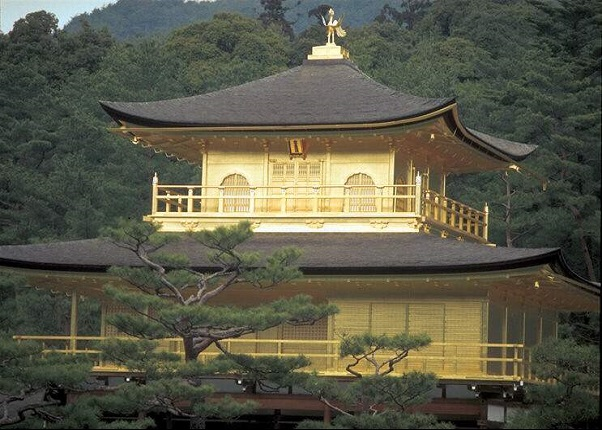
\includegraphics[scale=.5]{welcome.png}\\
\caption{Home Page}
\vspace{0.2 cm}
\justify
{This is home window of our project. It consist of two panels}\\
{1.Student panel-Through this panel student can perform his operations like registration and filling the feedback form. }\\
{2.Admin panel-Through this panel admin can perform his operations like registration,Faculty registration and display faculty rating}
\end{center}
\end{figure}
\begin{figure}[ht]
\begin{center}
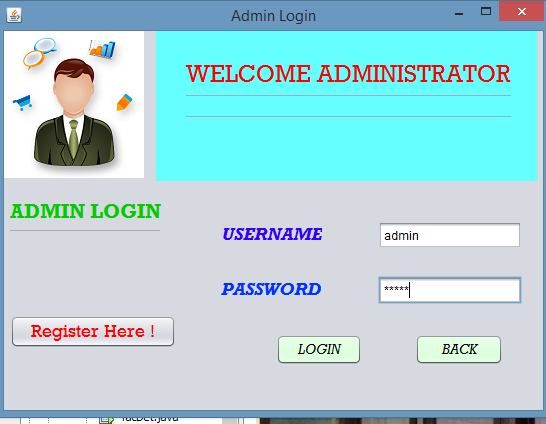
\includegraphics[scale=.7]{adminlogin.png}\\
\caption{Admin Login}
\vspace{0.2 cm}
\justify
{Through this window admin is authenticate and logged into the system.}
\end{center}
\end{figure}
\begin{figure}[ht]
\begin{center}
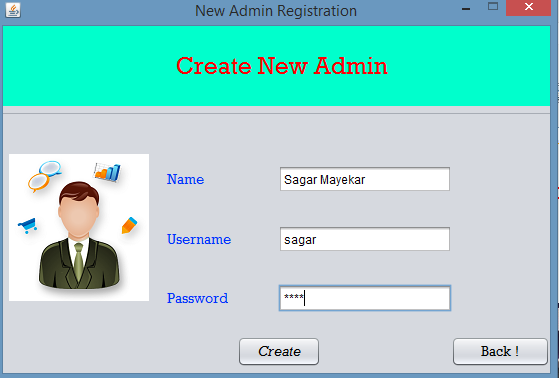
\includegraphics[scale=.7]{adminreg.png}\\
\caption{Admin Registration}
\vspace{0.2 cm}
\justify
{Through this window we can create new administrator for our system.}
\end{center}
\end{figure}
\begin{figure}[ht]
\begin{center}
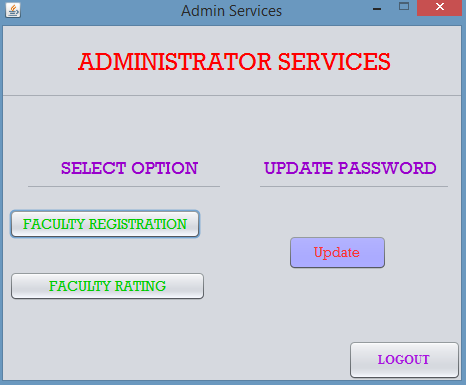
\includegraphics[scale=.7]{adminservice.png}\\
\caption{Admin Services}
\vspace{0.2 cm}
\justify
{Administrative services are:}\\
{1.Faculty Registration-Admin can register faculty through this window. }\\
{2.Faculty Rating-Admin can view the rating of particular faculty through this window.}\\
{3.Update Password- Admin can change his password from this window.}
\end{center}
\end{figure}
\begin{figure}[ht]
\begin{center}
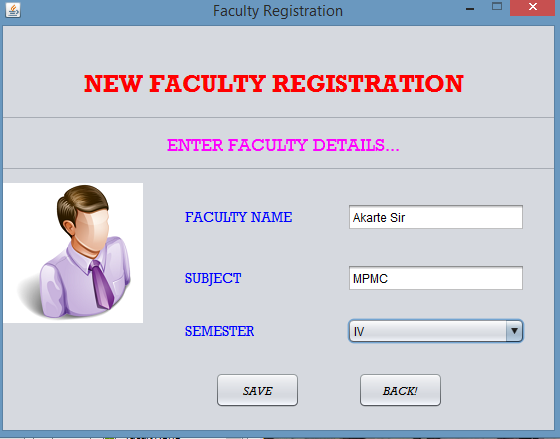
\includegraphics[scale=.7]{facultyreg.png}\\
\caption{Faculty Registration}
\vspace{0.2 cm}
\justify
{From this window Admin can register the new faculty for the respective subject and semester.}
\end{center}
\end{figure}
\begin{figure}[ht]
\begin{center}
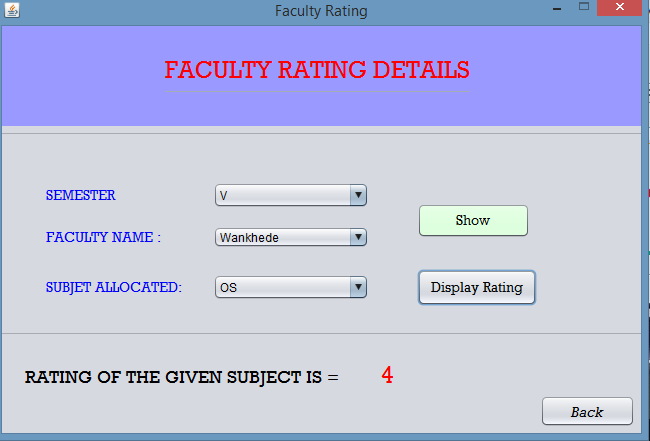
\includegraphics[scale=.7]{rating.png}\\
\caption{Faculty Rating}
\vspace{0.2 cm}
\justify
{From this window admin can see  What is the rating of that faculty.}
\end{center}
\end{figure}
\begin{figure}[ht]
\begin{center}
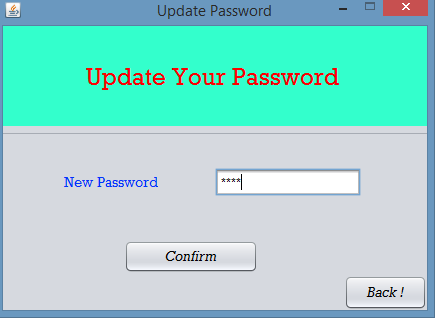
\includegraphics[scale=.7]{updatepass.png}\\
\caption{Admin Passupdate}
\vspace{0.2 cm}
\justify
{From this window admin can change his password.}
\end{center}
\end{figure}
\begin{figure}[ht]
\begin{center}
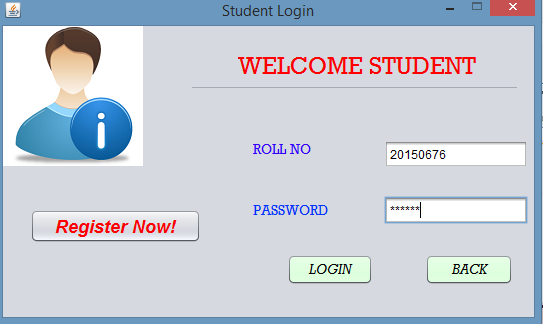
\includegraphics[scale=.7]{studlogin.png}\\
\caption{Student Login}
\vspace{0.2 cm}
\justify
{From this window student can logged into the system and fill the feedback for the every faculty.}\\
{Register Now- It redirect to the new student registration.}
\end{center}
\end{figure}
\begin{figure}[ht]
\begin{center}
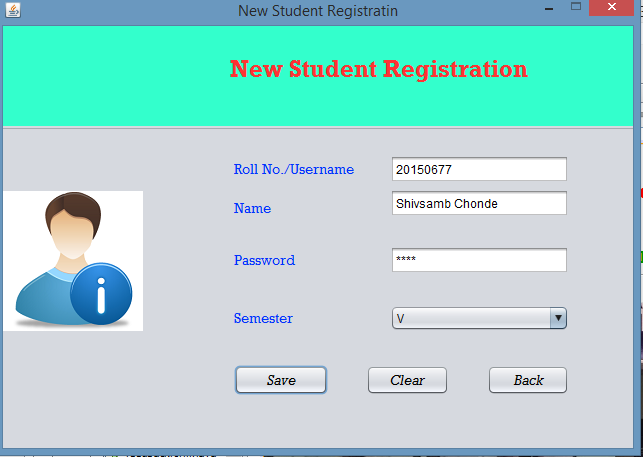
\includegraphics[scale=.7]{studreg.png}\\
\caption{Student Registration}
\vspace{0.2 cm}
\justify
{From this window we can register new student with user name and password also.}
\end{center}
\end{figure}
\begin{figure}[ht]
\begin{center}
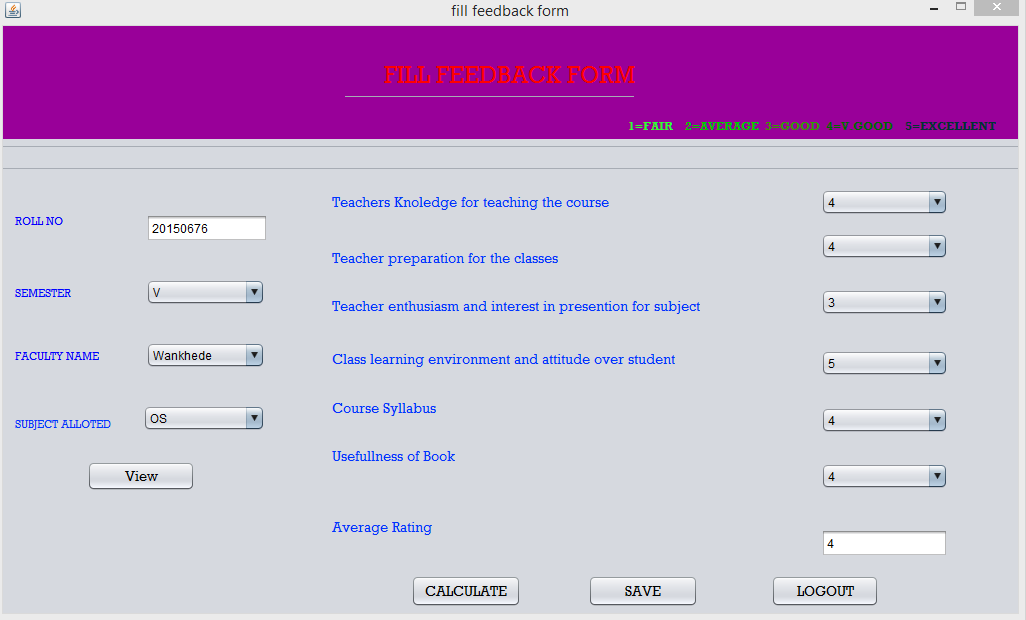
\includegraphics[scale=.5]{feedback.png}\\
\caption{Feedback Form}
\vspace{0.2 cm}
\justify
{After student logged into the system then This window will be open for the filling the feedback form.}
\end{center}
\end{figure}




\end{center}

\chapter{MAPPING REQUIREMENTS MODEL TO ARCHITECTURE MODEL}
\rule{\textwidth}{2 pt}
\section{Data Flow Diagram}
\subsection{Level-0 DFD }
\begin{figure}[ht]
\begin{center}
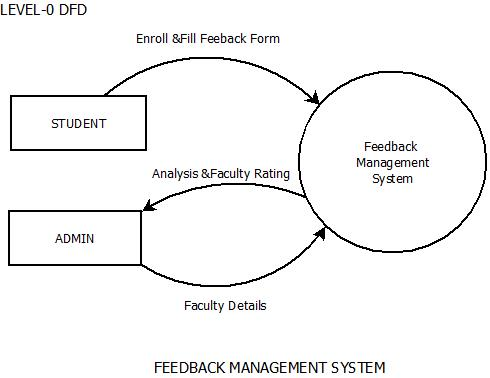
\includegraphics[scale=.6]{L-0.png}\\
\caption{Level-0 DFD}
\end{center}
\end{figure}
\subsection{Level-1 DFD }
\begin{figure}[ht]
\begin{center} 
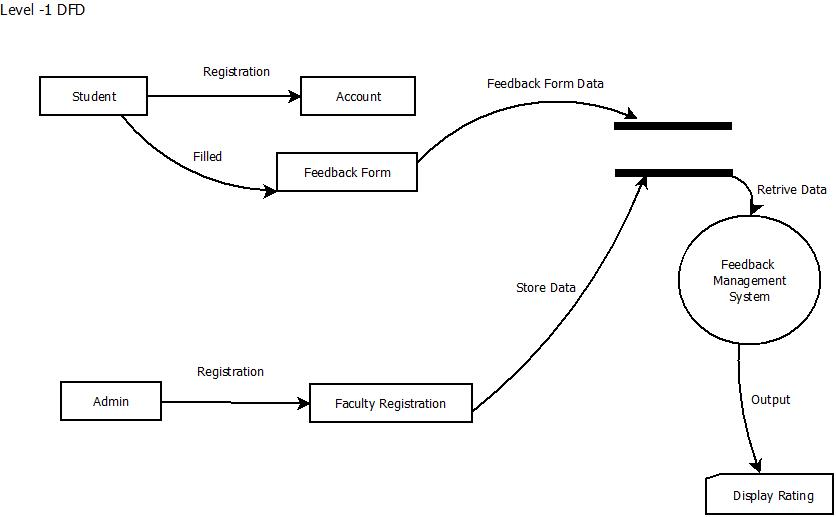
\includegraphics[scale=.4]{L-1.png}\\
\caption{Level-1 DFD}
\end{center}
\end{figure}
\subsection{Level-2 DFD }
\begin{figure}[ht]
\begin{center}
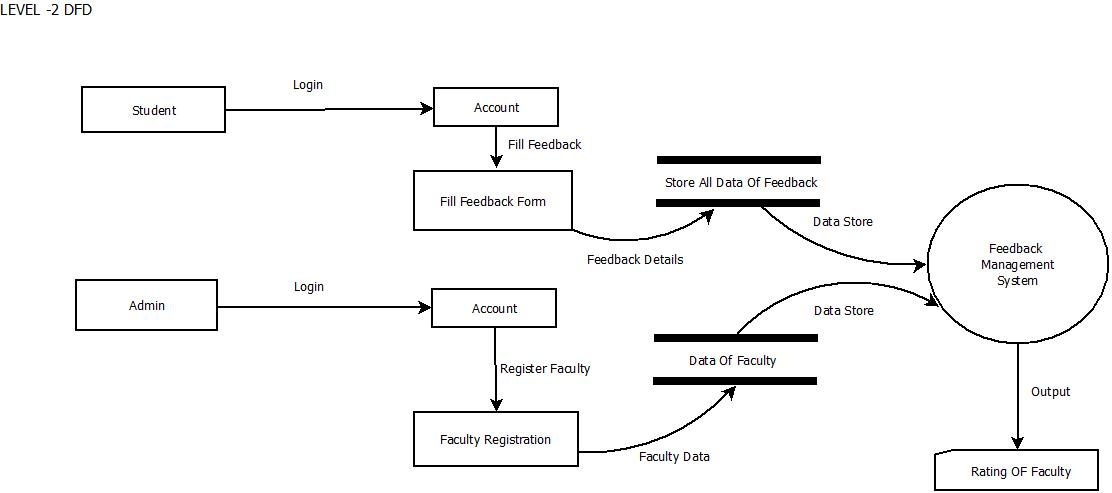
\includegraphics[scale=.4]{L-2.png}\\
\caption{Level-2 DFD}
\end{center}
\end{figure}

\newpage
\section{Sequence Diagram}
\begin{figure}[ht]
\begin{center}
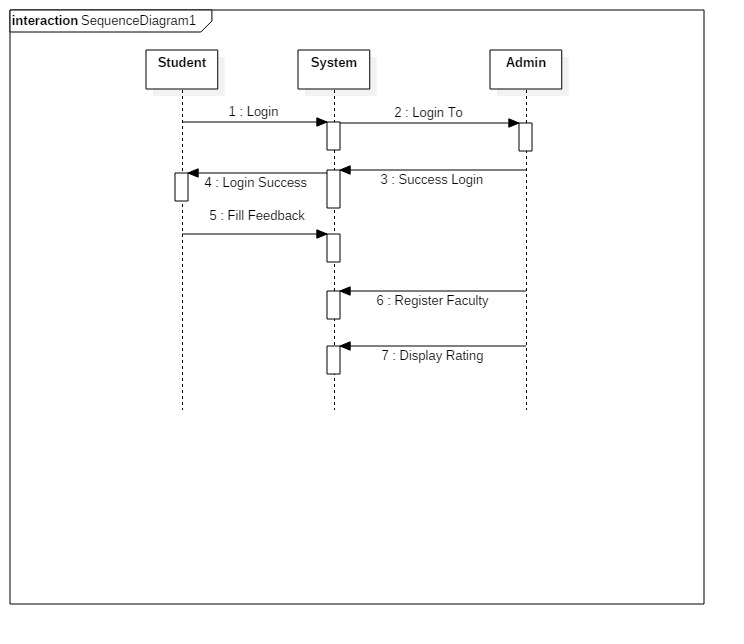
\includegraphics[scale=.5]{SequenceDiagram1new.png}\\
\caption{Sequence diagram}
\end{center}
\end{figure}
\newpage
\section{Usecase Diagram}
\begin{figure}[ht]
\begin{center}
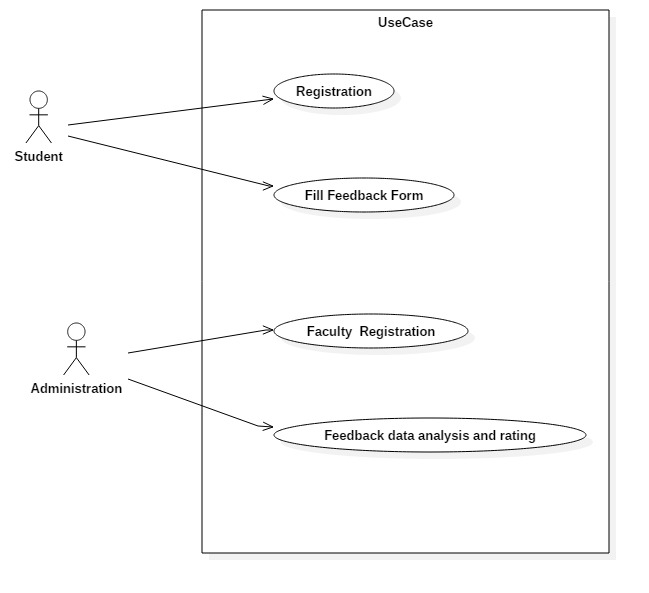
\includegraphics[scale=.5]{UseCaseDiagram1.png}\\
\caption{Usecase diagram}
\end{center}
\end{figure}
\newpage
\section{Activity Diagram}
\begin{figure}[ht]
\begin{center}
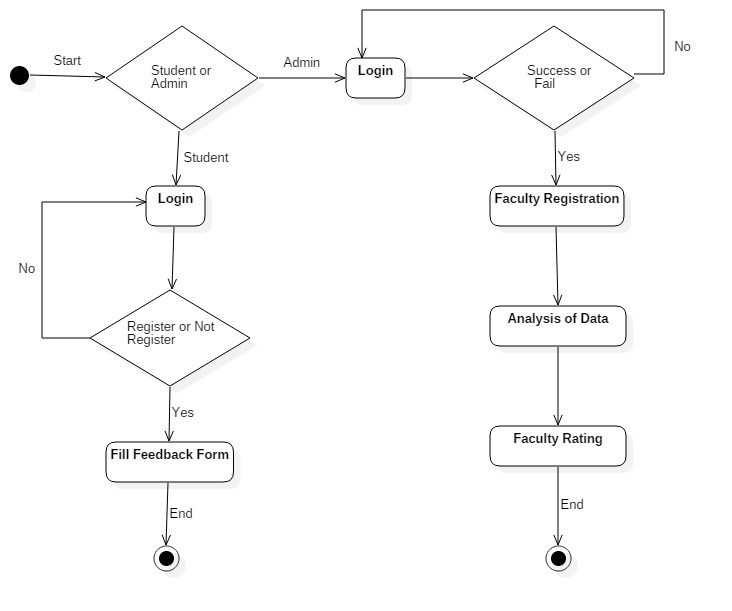
\includegraphics[scale=.5]{ActivityDiagram1.png}\\
\caption{Activity diagram}
\end{center}
\end{figure}
\newpage
\section{Swim Lane Diagram}
\begin{figure}[ht]
\begin{center}
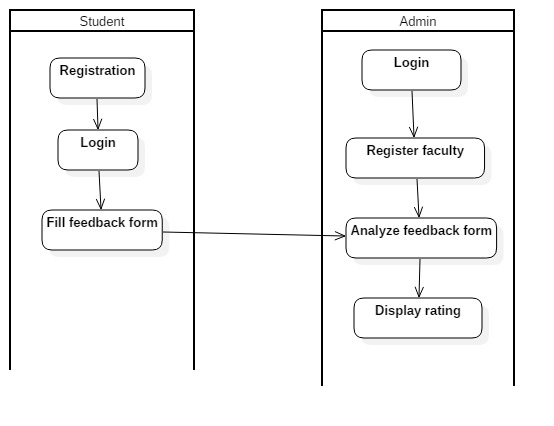
\includegraphics[scale=.5]{swim.png}\\
\caption{Swim Lane diagram}
\end{center}
\end{figure}
%\end{comment}

\chapter{SYSTEM REQUIREMENT SPECIFICATION}

\rule{\textwidth}{2 pt}
\justify
\section{Technical Requirement}
1.Netbeans IDE(8.0 and above)\\
2.Oracle DB(10g XE)\\
3.Windows based OS
\section{User Requirement}
1.Fully automated\\
2.Better GUI\\
3.Less time consuming\\
4.Well analyzed
\chapter{ADVANTAGES \& APPLICATIONS}
\rule{\textwidth}{2 pt}
\justify
\section{Advantages}
1.Provide automation for existing system.\\
2.Automated process for filling feedback form.\\
3.Easy access to the data.
\section{Application}
1.Use in department of computer engineering 
\chapter{FUTURE ENHANCEMENT}
\begin{center}
\rule{\textwidth}{2 pt}
\justify
1.We can display faculty and subject according to semester.\\
2.We can develop system for other departments of college also.\\
3.There should be separate registration for permanent and adhoc faculty.
\end{center}
\chapter{CONCLUSION}
\begin{center}
\rule{\textwidth}{2 pt}
\justify
Today the technology is beyond what we could imagine before. Also now-a-days, the new developments are not just the result of the necessity, rather invention and innovation are the new drivers in the development of technology. So constant updation is the key method to stay and survive in the emerging market of science and technology.The new  software that we developed ie. Feedback management system that has been proposed practically implemented for use in computer engineering department management field. Our imaginations have dressed into reality and with the new concept.\\
Proposed system is automated and advance than existing system because it maintain,store and analyze data very efficiently.

\end{center}

\chapter{BIBLIOGRAPHY}
\begin{center}
\rule{\textwidth}{2 pt}
\justify
\section{Websites}
{1.https://www.tutorialspoint.com/java}\\
{2.https://www.javatpoint.com/java-tutorial}\\
{3.https://dcs.oracle.com/javas}\\
{4.https://www.w3schools.com}
\section{Boooks}
{1.Java programming by Sarita Gaikwad,Tech-Max publication.}\\
{2.Java:The Complete Reference by Herbert Schildt,The McGraw-Hill Companies.}

\end{center}

\end{document}

\end{document}